\lysh{24363}{4}
\begin{alist}
\item Για $x \in \mathbb{R}$ η συνάρτηση $f$ είναι παραγωγίσιμη με:
\[ f'(x) = \left( \frac{x}{x^2+1} \right)' = \frac{(x)'(x^2+1) - x \cdot (x^2+1)'}{(x^2+1)^2} = \frac{x^2+1 - x \cdot 2x}{(x^2+1)^2} = \frac{1-x^2}{(x^2+1)^2}. \]

\item Λόγω του ερωτήματος ($\alpha$) η $f'(x) = \frac{1-x^2}{(x^2+1)^2}$, $x \in \mathbb{R}$.

Είναι $f'(x) = 0 \Leftrightarrow 1-x^2 = 0 \Leftrightarrow x=-1 \text{ ή } x=1$ και $f'(x) > 0 \Leftrightarrow 1-x^2 > 0 \Leftrightarrow -1 < x < 1$.

\begin{center}
\begin{tikzpicture}
\tikzset{arrow style/.style={maincolor,>->,>=latex'}}
\tikzset{t style/.style = {style = dashed}}
\tikzset{z style/.style = {fill=white,inner sep=.2mm}}
\tkzTabInit[color,lgt=2,espcl=2.4,colorC = maincolor!50,colorL = maincolor!30,colorV = maincolor!50]%
{$x$ / .8,$f'$ /.8,$f$/1.2}%
{$-\infty$,$-1$,$1$,$+\infty$}%
\tkzTabLine{,-,z,+,z,-,}
\tkzTabVar{+/ , -/ \text{TE} , +/ \text{TM} , -/ }
\end{tikzpicture}
\end{center}

Επομένως η συνάρτηση $f$ είναι γνησίως φθίνουσα στο διάστημα $(-\infty,-1]$, γνησίως αύξουσα στο διάστημα $[-1,1]$ και γνησίως φθίνουσα στο διάστημα $[1,+\infty)$.

Για $x=-1$ η συνάρτηση $f$ παρουσιάζει τοπικό ελάχιστο ίσο με $f(-1) = -\frac{1}{2}$

και για $x=1$ παρουσιάζει τοπικό μέγιστο ίσο με $f(1) = \frac{1}{2}$.

\item Είναι $f(2) = \frac{2}{5}$ οπότε το $\mathrm{M}(2, f(2)) = \left(2, \frac{2}{5}\right)$.

Λόγω του ερωτήματος ($\alpha$) η $f'(2) = \frac{1-2^2}{(2^2+1)^2} = -\frac{3}{25}$.

Έστω $(\varepsilon): y = \lambda x + \beta$ με $\lambda,\beta \in \mathbb{R}$, η εφαπτομένη της γραφικής παράστασης της συνάρτησης $f$ στο σημείο $\mathrm{M}$.

Είναι $\lambda = f'(2) = -\frac{3}{25}$, οπότε η $(\varepsilon): y = -\frac{3}{25}x + \beta$.

Επίσης το $\mathrm{M}\left(2, \frac{2}{5}\right) \in (\varepsilon) \Leftrightarrow \frac{2}{5} = -\frac{3}{25} \cdot 2 + \beta \Leftrightarrow \beta = \frac{2}{5} + \frac{6}{25} = \frac{16}{25}$.

Επομένως $(\varepsilon): y = -\frac{3}{25}x + \frac{16}{25}$.
\end{alist}
\vspace{6mm}
\noindent\rule{\textwidth}{0.4pt}
\vspace{6mm}

